%!TEX root = /Users/dbreuer/Documents/Work/_FH/_Master/master_thesis/Main/Master Thesis.tex

\chapter{COSIMA - Eine dienstorientierten Multimediaarchitektur} % (fold)
\label{cha:eine_dienstorientierten_multimediaarchitektur}

  Im Abschnitt~\ref{sec:motivation} wurde bereits kurz darauf eingegangen, dass die vorliegenden Arbeit vor dem Hintergrund des COSIMA-Projekts entstanden ist. In diesem Kapitel soll dieses Projekt so weit vorgestellt werden, dass für den weiteren Verlauf der Arbeit ein grundlegendes Verständnis über die Ziele, Alleinstellungsmerkmale und Herausforderungen existiert.
  
\section{Motivation und Ziele von COSIMA} % (fold)
\label{sec:motivation_und_ziele_von_cosima}

  Das COSIMA-Projekt ist aus dem Wahlpflichtfach Modellierung in audio-visuellen Medien (MIAV\abk{MIAV}{Modellierung in audio-visuellen Medien}) an der Fachhochschule Köln im Masterstudiengang der Medieninformatik hervorgegangen. Im Rahmen einer Projektarbeit wurde das die Projektidee weiter ausgearbeitet und konzeptioniert. Die Ergebnisse dieser Arbeit wurden als Institutsbericht an Fachhochschule Köln bereitsgestellt und sind dort im Detail einsehbar~\citep{bericht}.
  
  Das folgende Kapitel wird daher nur auf die wesentliche Punkte des COSIMA-Projekts eingehen und ihre Relevanz für diese Arbeit herausstellen. Die ursprüngliche Idee hinter COSIMA war es ein Framework zu entwickeln, dass die Entwicklung von Multimediaanwendungen vereinfacht. Im Gegensatz zu anderen Medienframeworks, wie etwa dem \emph{Java Media Framework} (JMF\abk{JMF}{Java Media Framework}), wurde bei dem COSIMA-Projekt ein ganzheitlicher Ansatz verfolgt.
  
  Im Institutsbericht wird darauf hingewiesen, "`dass die Entwicklung von Multimediaanwendungen derzeit verhältnismässig aufwendig ist"'~\citep[S. 2]{bericht}. Eine Ursache dieser Problematik, liegt nach Aussage der Autoren darin begründet, dass sich die zur Zeit verfügbaren Rahmenwerke im Bereich der Multimediaverarbeitung auf einen sehr engen Einsatzbereich beschränken. Neben JMF sind hier zusätzlich noch \emph{QuickTime}\footnote{\url{http://www.apple.com/quicktime/}} und \emph{ImageJ}\footnote{\url{http://rsbweb.nih.gov/ij/}} zu nennen. Andere Aspekte von Multimediaanwendungen, wie etwa die Integration von Metadaten, müssten von dem Anwendungsentwickler erst manuell mit diesen Rahmenwerken integriert werden. "`Ein Meta-Framework, welches die bestehenden Ansätze verbinden und integrieren könnte, würde die Wiederverwendbarkeit und generelle Entwicklungsarbeit positiv beeinflussen, beziehungsweise vereinfachen"'~\citep[S. 3]{bericht}, wird von den Autoren des Berichts daher als Bestreben hinter dem COSIMA-Projekt angeführt.
  
  Neben der Notwendigkeit ein \emph{Meta-Framework}\footnote{Das ursprüngliche Ziel war tatsächlich ein Framework zu schaffen. Erst während der Validierung im Rahmen dieser Arbeit ist zu Tage gekommen, dass es sich mehr um eine Architektur handelt und weniger um ein Framework. Im weiteren Verlauf wird darauf jedoch noch genauer eingegangen.} zu schaffen, führen die Autoren als weiteren Beweggrund das Fehlen einer Architektur für Multimediaanwendungen an. Innerhalb dieser Architektur könnten sich Anwendungsentwickler wesentlicher effektiver bewegen und müssten nicht erst eine eigene Architektur von Grund auf entwerfen.
  
  Da sich mit den meisten bestehenden Multimedia-Rahmenwerke keine verteilten Anwendungen realisieren lassen, lag auch dieser Aspekt von Beginn an im Fokus der Konzeptionierung. Als Grundlage eine geeignete Architektur zu konzeptionieren, die es ermöglicht, verteilte Anwendungen zu realisieren, diente das Konzept der \emph{Service-oriented Architecture} (SOA\abk{SOA}{Service-oriented Architecture}) oder \emph{Dienst-orientierten Architektur}.
  
  Die hier aufgeführten Punkte haben initial die Entwicklung eines Rahmenwerkes motiviert, dass später im COSIMA-Projekt aufgehen sollte. Die im Verlauf der Projektarbeit entwickelten Ziele von COSIMA sind im nächsten Abschnitt zusammen gefasst.
  
\subsection{Ziele} % (fold)
\label{sub:ziele}

  Das \emph{Mission Statement} des COSIMA-Projekts fasst alle Ziele des Projekts in einer Kernaussage zusammen:

  \begin{quote}
    \emph{``MIAV ist ein integratives, komponentenbasiertes Meta-Framework mit gezielter Ausrichtung auf Multimediaverarbeitung. Es vereinfacht die Entwicklung von verteilten Multimedia-Applikationen durch eine flexible, dienst-orientierte Architektur. Die Wiederverwendbarkeit von Komponenten und bestehenden Frameworks wird dadurch begünstigt.''} (aus~\citep[S. 2]{bericht})\footnote{Die Bezeichnung "`COSIMA"' hat das Projekt erst nach Fertigstellung des Berichts erhalten, daher findest sich hier noch die zuvor verwandte provisorische Bezeichnung \emph{MIAV-Framework}.}
  \end{quote}

  Neben den zentralen Aspekten \emph{dienst-orientierte Architektur}, \emph{Integration} und \emph{Meta-Framework}, die im Abschnitt zuvor bereits dargestellt wurden, nennen die Autoren hier zusätzlich noch die Aspekte der \emph{komponentenbasierten Architektur}, \emph{Wiederverwendbarkeit} und natürlich der \emph{Medienverarbeitung}.
  
  Neben den hier genannten Zielen, die das COSIMA-Projekt zu erreichen versucht, zeichnet sich das Projekt durch seine spezifischen Charakteristika in Bezug auf andere Multimedia-Rahmenwerke aus. Diese Alleinstellungsmerkmale werden im nächsten Abschnitt genauer betrachtet.

  % - Welche Ziele verfolgt das COSIMA-Projekt?
  % - Warum handelt es sich um eine Architektur und nicht um ein Framework!!!! (Im Bericht noch anders, irgendwie muss das hier verwurstet werden!)
  % - Weiterentwicklung der Definition seit dem Bericht

% subsection ziele (end)
  
% section motivation_und_ziele_von_cosima (end)

\section{Alleinstellungsmerkmale} % (fold)
\label{sec:alleinstellungsmerkmale}

  Aus den in Abschnitt~\ref{sub:ziele} dargestellten Zielen des COSIMA-Projekts lassen sich die folgenden Merkmale extrahieren, die COSIMA im Bereich der Multimedia-Rahmenwerke und -Anwendungen einmalig machen~\citep[S. 3f]{bericht}:
  
  \begin{description}
    \item[Verteiltheit] COSIMA ist konzeptioniert als ein verteiltes System.
    \item[Dienstorientierung] Angelehnt an die \emph{Service-Oriented Architecture} (SOA), sind die Bausteine in COSIMA als Dienste modelliert.
    \item[Integration] Bestehende Frameworks können in Form von Diensten angeboten und so ihre Funktionalität eingebunden werden.
    \item[Erweiterbarkeit] Die Dienstorientierung erlaubt die Einbindung eigener Komponenten.
    % TODO - Die Skalierbarkeit muss hier noch weiter beschrieben werden. Eine reine Verteilung führt noch zu keiner gute Skalierbarkeit eines Systems.
    \item[Skalierbarkeit] Als verteiltes System können Dienste auf verschiedene Systeme ausgelagert werden, es gibt kein monolithisches System\footnote{die Verschiebung des Flaschenhalses von einem System hat zur Folge, dass die Verbindung zwischen den Diensten entsprechend angelegt sein muss. [\textbf{QUELLE}]}.
    \item[Medienobjekt-Modellierung] Modellierung von Medien in ganzheitlicher Betrachtungsweise von Rohdaten und Metadaten in einem Objekt.
    \item[Meta-Ebene] COSIMA fokussiert nicht auf Datensicht oder Metadatensicht sondern abstrahiert auf höhere Ebene.
    \item[Medienverarbeitung] Ganzheitliche Sicht auf Medienverarbeitung: Produktion, Verarbeitung, Transformation, Anreicherung, Wiedergabe, Ausgabe von Daten und Metadaten
    \item[Architektur] COSIMA stellt eine Architektur für Multimediaanwendungen
  \end{description}
  
  Basierend auf den vorgestellten Zielen und Alleinstellungsmerkmalen wurde die Architektur entworfen, die in dieser Arbeit validiert und prototypisch realisiert wurde. Im Folgenden Abschnitt wird diese Architektur im Detail vorgestellt werden.

% section alleinstellungsmerkmale (end)

\section{Architektur} % (fold)
\label{sec:architektur}

  Die Architektur des COSIMA-Projekts ist iterativ in einem dedizierten Vorgehen\footnote{Dieses Vorgehen wird detailliert im Institutsbericht vorgestellt. Eine Erläuterung in diesem Rahmen ist nicht angemessen und wird daher ausgelassen.} bis zu dem Punkt entwickelt worden, der als Ausgangspunkt für die Betrachtungen in dieser Arbeit dient.

\subsection{Einführung} % (fold)
\label{sub:einfuehrung}

  Bei der Konzeption und Entwicklung der Architektur sind unterschiedliche Sichten auf diese erstellt worden. Diese Sichten entsprechen denen von Starke in~\citep[S. 83]{effektive_software_architekturen} beschriebenen vier Arten von Sichten auf eine Software-Architektur: \emph{Kontextsichten}, \emph{Bausteinsichten}, \emph{Laufzeitsichten} und \emph{Verteilungssichten}.

  Für das COSIMA-Projekt wurden bisher Darstellungen aus zwei dieser Kategorien erstellt: eine der Kontextsichten und drei der Bausteinsichten. Die Kontextsichten legen laut Starke den "`Fokus auf den Zusammenhang oder das Umfeld des Systems"'~\citep[S. 87]{effektive_software_architekturen}, was auch auf die in Abbildung~\ref{fig:images_Kontextsicht_Architektur_COSIMA} dargestellte Kontextsicht von COSIMA zutrifft. Hier wird lediglich ein abstrakter und vor allem nicht formaler Überblick über die Architektur und beteiligte Systeme gegeben. Die Darstellungen, die sich den Bausteinsichten zuordnen lassen, sind namentlich das \emph{Komponentendiagramm}, das \emph{Kompositionsstrukturdiagramm} und der \emph{Grobentwurf} der Architektur. Diese finden sich jeweils in~\citep{bericht} und sollen an dieser Stelle nicht weiter betrachtet werden\footnote{\textbf{TODO}: Im weiteren Verlauf werden sicher Teile aus diesen Diagrammen benötigt, daher muss dann darauf referenziert werden.}. Für die weitere Vorstellung der Architektur soll an dieser Stelle die Kontextsicht genügen.

\begin{figure}[ht]
  \centering
    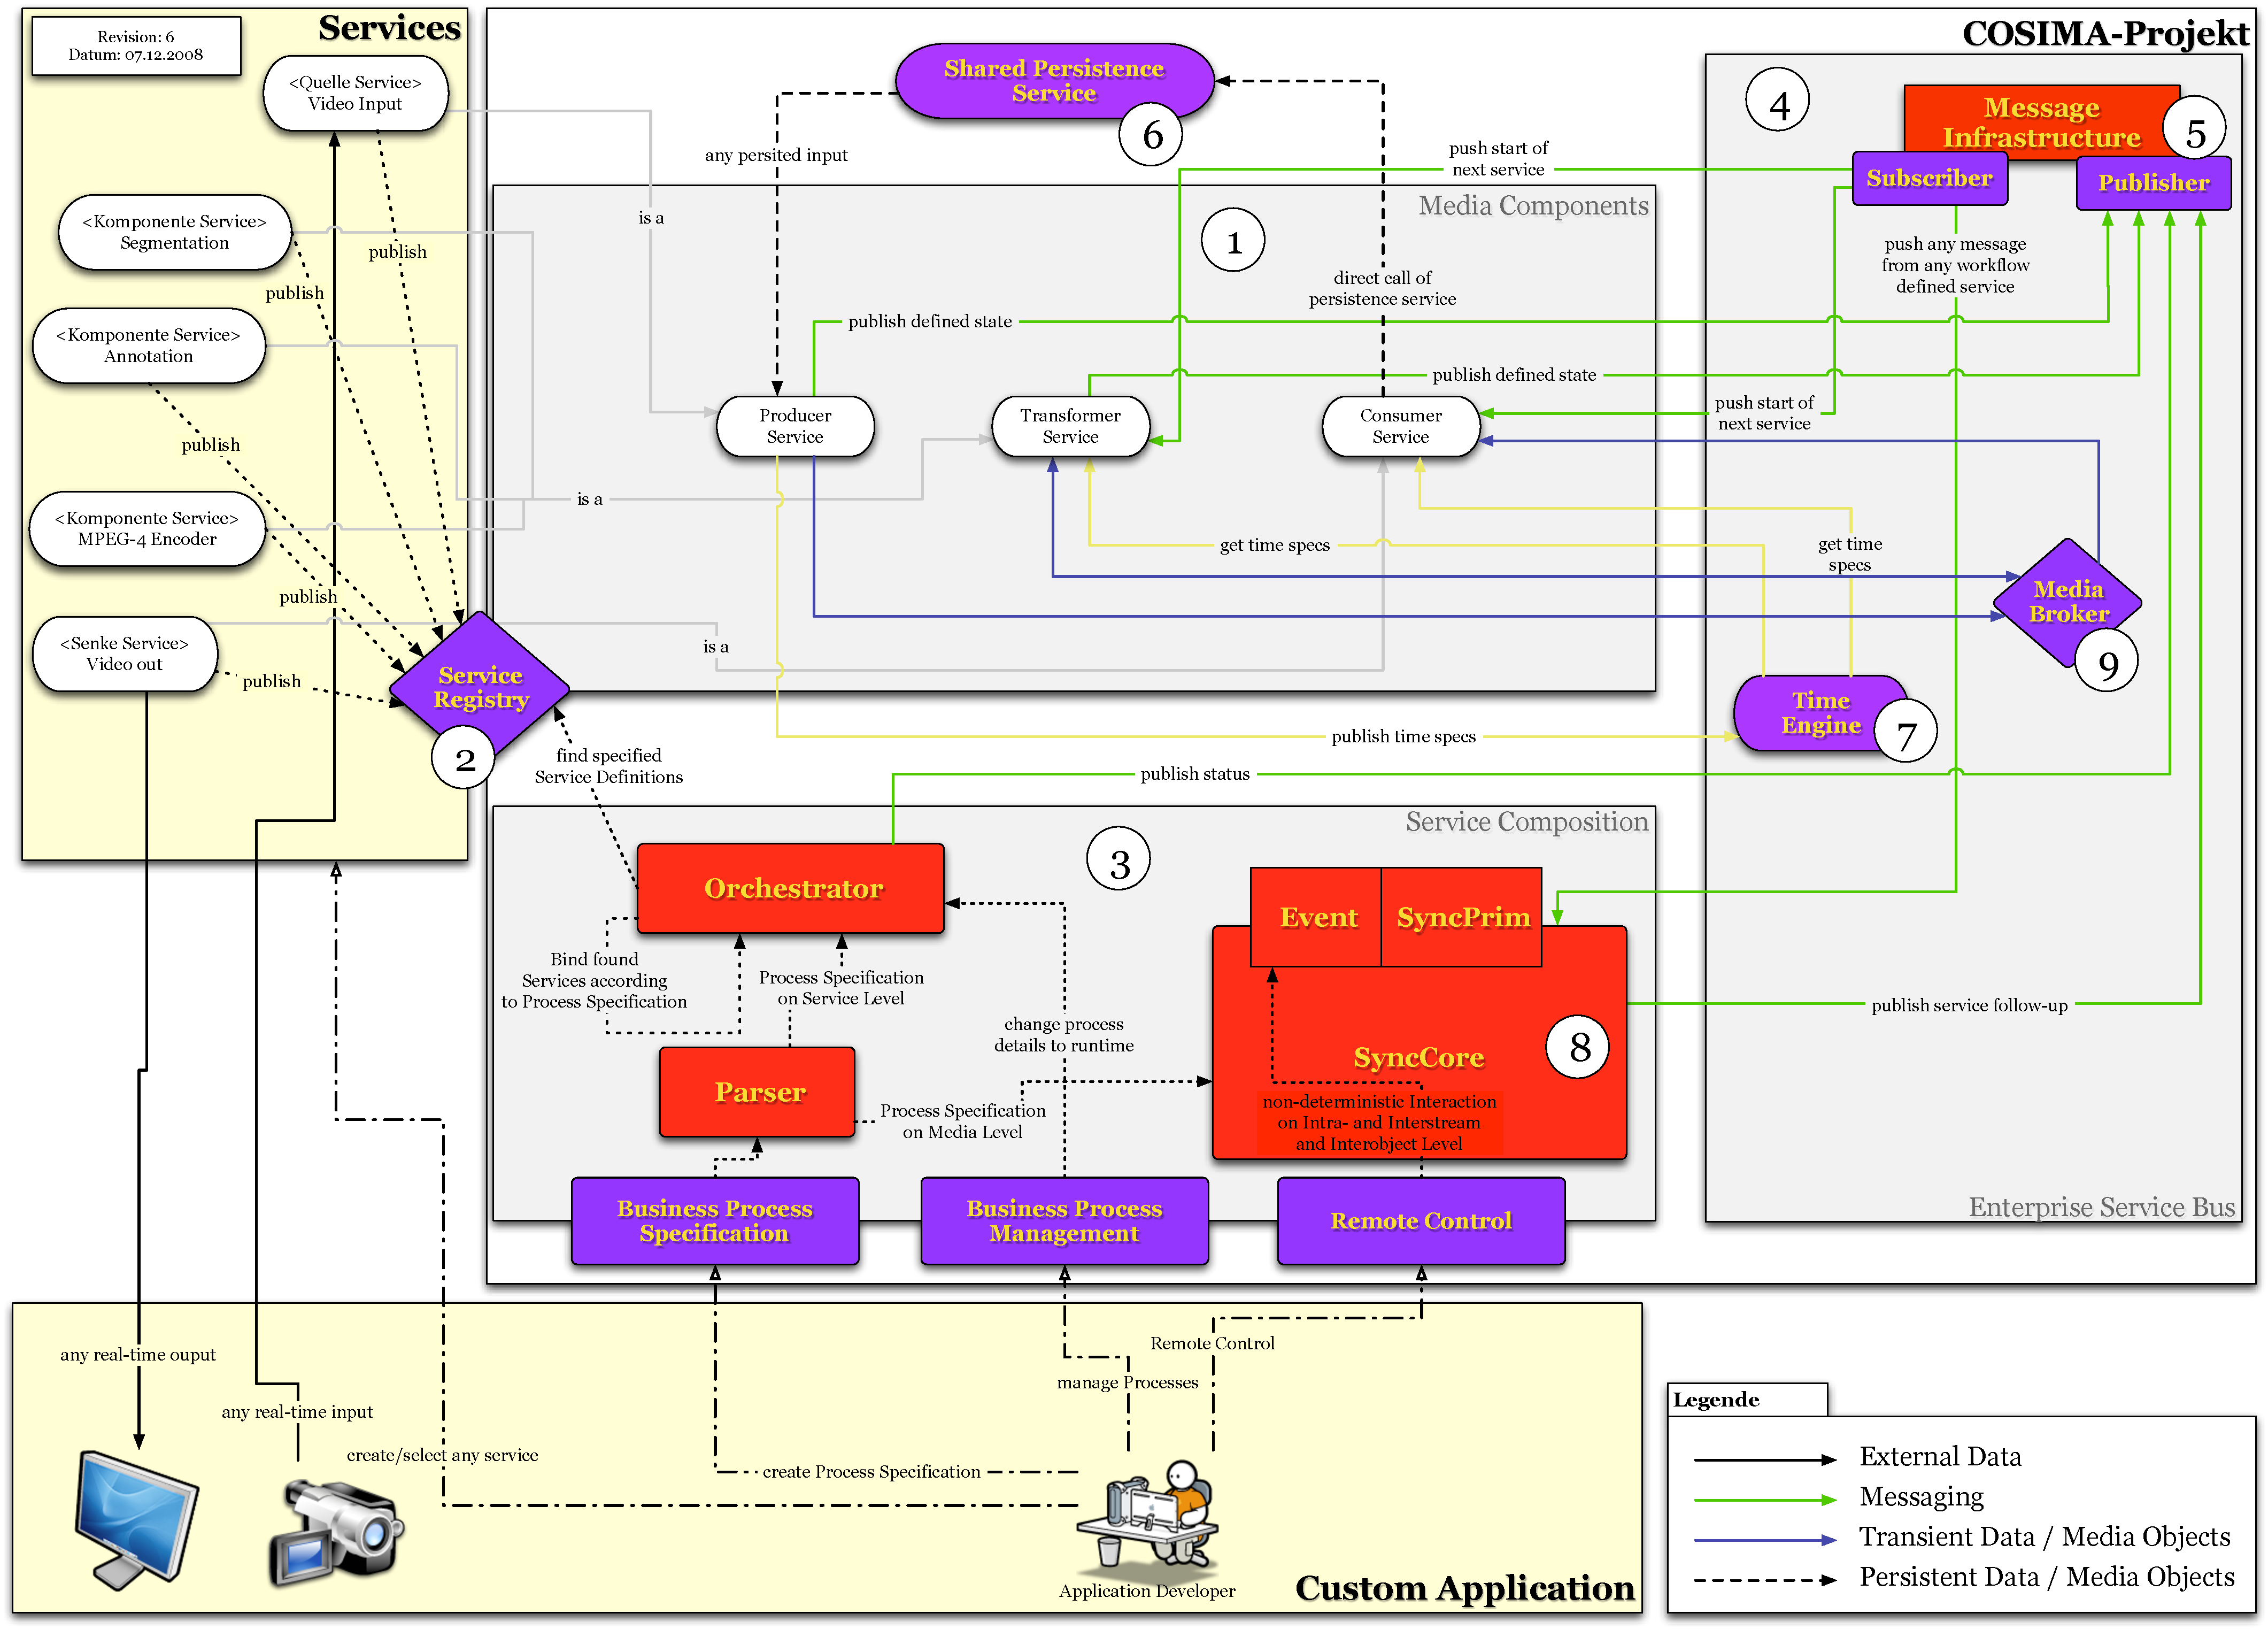
\includegraphics[width=.9\textwidth]{images/Kontextsicht_Architektur_COSIMA}
  \caption{Kontextsicht der Architektur des COSIMA-Projekts}
  \label{fig:images_Kontextsicht_Architektur_COSIMA}
\end{figure}

  In der späteren prototypischen Realisierung und anschließenden Validierung der Architektur sollen und können nur Fragmente der Architektur umgesetzt werden, daher ist es sehr wichtig, solche Fragmente zu wählen, die für eine Weiterentwicklung von besonderem Interesse sind. Im Folgenden werden daher die zentralen Komponenten des COSIMA-Projekts kurz vorgestellt. \emph{Später soll dann eine Auswahl getroffen werden.}

  % - Kernpunkte der Architektur herausarbeiten
  % - Diese Kernpunkte müssen in der Realisierung/Validierung entsprechend besondere Berücksichtigung finden

% subsection einfuehrung (end)

\subsection{Medienverarbeitende Komponenten} % (fold)
\label{sub:medienverarbeitende_komponenten}

  Den Kern von COSIMA machen die medienverarbeitenden Komponenten aus, die vom Anwendungsentwickler in eine entsprechende Abfolge gebracht werden und damit die später Multimediaanwendung selbst darstellen: \emph{Producer}, \emph{Transformer} und \emph{Consumer}. Dem Entwurf der Komponenten liegt das \emph{Quelle-Komponente-Senke} Prinzip zu Grunde. Die innerhalb des COSIMA-Projekts verwendete Bezeichnung ist nach~[\textbf{QUELLE}] ebenso valide wie die geläufigere Bezeichnung "`Quelle-Komponente-Senke"'. Da es sich bei COSIMA jedoch um eine komponentenbasierte Architektur handelt, bot sich die Alternative Bezeichnung weit mehr an.
  
  Diese medienverarbeitenden Komponenten sind alle als Dienste ausgeprägt, um dem Anspruch der Dienstorientierung gerecht zu werden. Eine Komponente kann dabei niemals eine andere Komponente direkt aufrufen, diese Aufgabe obliegt der \emph{Service Komposition} (siehe Abschnitt~\ref{sub:service_komposition}). Jede dieser Komponenten muss sich dazu bei seiner Initiierung beim Service Repository registrieren, der in~\ref{sub:service_registry} näher beschrieben wird.
  
  Der Austausch der zu verarbeitenden Medien zwischen den einzelnen Komponenten geschieht auschließlich über den \emph{Media Broker}, der unter~\ref{sub:medienobjekt} weiter ausgeführt wird. Ein genereller Nachrichtenaustausch unter den Komponenten im speziellen und mit den restlichen Elementen der Architektur wird über das Nachrichtensystem (\ref{ssub:nachrichtensystem}) realisiert. Persistenz von Daten und die Synchronisation werden von einem \emph{Persistence Data Service} bzw. der \emph{Timing Engine} übernommen. Beide Komponenten werden in~\ref{sub:infrastruktur} näher beschrieben. Teile dieser Architekturelemente sollen einmal in einem Service Bus aufgehen~\citep[S. 18]{bericht}.

% subsection medienverarbeitende_komponenten (end)

\subsection{Service Registry} % (fold)
\label{sub:service_registry}

  Die Service Registry ist nach~\citep{service_oriented_computing}, als konstituierendes Element innerhalb einer SOA, selbst wieder ein Dienst, der die Dienstbeschreibungen anderer Dienste vorhält und bereitstellt. Jeder Dienst innerhalb von COSIMA muss daher seine Beschreibung bei der Service Registry bekannt machen. Es kann demnach auch keinen anderen Weg geben als über die Service Registry eine Verbindung zu einem Service aufzunehmen.

  % - Zentrale Stelle zur Registrierung/Auffindung von Services
  % - Definition der allgemeinen Schnittstelle für COSIMA-Services

% subsection service_registry (end)

\subsection{Service Komposition} % (fold)
\label{sub:service_komposition}

  - Definitionen von "`Workflow"' und "`Prozess"' in Zusammenhang auf die Entwürfe (vielleicht )
  - BPEL/Orchestrierung/Choreographie mit Quellenangaben erläutern
  - vielleicht macht dieser Abschnitt überhaupt keinen Sinn!
  - Die grundsätzliche Möglichkeit der Verwendung einer Prozessbeschreibungssprache diskutieren

% subsection service_komposition (end)

\subsection{Infrastruktur} % (fold)
\label{sub:infrastruktur}

  - Beschreibung der (abstrakten) Infrastrukturelemente
  - Eigentlich gehört auch das Medienobjekt grob zur Infrastruktur, ist jedoch so wichtig, dass es eigenen Punkt erhält

\subsubsection{Nachrichtensystem} % (fold)
\label{ssub:nachrichtensystem}

  - Verwendung
  - Einfluss auf Komposition

% subsubsection nachrichtensystem (end)

\subsubsection{Persistenz} % (fold)
\label{ssub:persistenz}

  - Persistenzschicht
  - jetzt nicht wichtig

% subsubsection persistenz (end)

\subsubsection{Timing} % (fold)
\label{ssub:timing}

  - gedacht für Synchronisation
  - auch nicht im Fokus der Betrachtungen

% subsubsection timing (end)

% subsubsection infrastruktur (end)

\subsection{Medienobjekt und Media Broker} % (fold)
\label{sub:medienobjekt}

  - Begründung warum separat betrachtet von Infrastruktur
  - Media Broker?!
  - Bedeutung für COSIMA
  - Verantwortlichkeiten

% subsection medienobjekt (end)

\subsection{Offene Fragen} % (fold)
\label{sub:offene_fragen}

  - Was ist zu diesem Zeitpunkt noch offen?
  - Was kann auch am Ende dieser Arbeit nicht abschließend geklärt sein?
  - Kann hier überhaupt noch von einem "`Framework"' gesprochen werden?

% subsection offene_fragen (end)

% section architektur (end)

% chapter eine_dienstorientierten_multimediaarchitektur (end)
